\chapter{Testy benchmarku}\label{chap:test_bench}

Omawiany w tej pracy benchmark został poddany szeregowi testów, począwszy od testów jednostkowych
pojedynczych klas i modułów, przez testy współpracy z różnymi DBMS, po testy mające na celu przyjrzenie się
uzyskiwanym wynikom przy różnej liczbie RTE. 

Testy jednostkowe zostały oparte o bibliotekę JUnit~\cite{JUnit1}. Ich pomyślne przejście było niezbędne do 
przeprowadzenia pozostałych testów. Testy te skupiały się głównie na sprawdzeniu poprawności działania pojedynczych 
klas czy modułów.

Drugą grupę stanowiły testy polegające na sprawdzeniu czy benchmark poprawnie przechodzi przez wszystkie kroki
procedury testowej dla dwóch wybranych modeli -- sklepu i hurtowni danych, oraz dla trzech różnych DBMS -- MySQL 5.0~\cite{MySql1},
PostgreSQL 8.1~\cite{PostgreSql1} i Oracle 10g~\cite{Oracle1}.

Trzecią grupę stanowiły testy wybranego DBMS przy stałym obciążeniu i zmiennej liczbie RTE. Niniejszy rozdział omawia właśnie
testy tego rodzaju.

\section{Środowisko testowe}
Omawiane w tym rozdziale testy zostały przeprowadzone na trzech komputerach A, B i C. Komputery te zostały połączone 
bezpośrednio siecią Fast Ethernet 100Mb/s. Konfiguracja komputerów została przedstawiona w tabelach \ref{tab:kompa},
\ref{tab:kompb} oraz \ref{tab:kompc}. 

\begin{table}[h]
\caption{Konfiguracja komputera A}\label{tab:kompa}
\begin{center}
\begin{tabular}{|l|l|}
\hline
Procesor&AMD Athlon 1.4 GHz\\
\hline
Pamięć RAM&512MB DDRAM\\
\hline
Dysk twardy&40GB\\
\hline
System operacyjny&Windows XP Professional SP2\\
\hline
\end{tabular}
\end{center}
\end{table}

\begin{table}[h]
\caption{Konfiguracja komputera B}\label{tab:kompb}
\begin{center}
\begin{tabular}{|l|l|}
\hline
Procesor&Pentium 2 350MHz\\
\hline
Pamięć RAM&320MB SDRAM\\
\hline
Dysk twardy&40GB Seagate Baracuda\\
\hline
System operacyjny&Windows XP Professional\\
\hline
\end{tabular}
\end{center}
\end{table}

\begin{table}[h]
\caption{Konfiguracja komputera C}\label{tab:kompc}
\begin{center}
\begin{tabular}{|l|l|}
\hline
Procesor&Pentium 3 700MHz\\
\hline
Pamięć RAM&128MB SDRAM\\
\hline
Dysk twardy&10GB\\
\hline
System operacyjny&Windows XP Professional\\
\hline
\end{tabular}
\end{center}
\end{table}

W testach wykorzystano bazę danych MySQL 5.1 -- została ona uruchomiona na komputerze A.
Przed każdym testem baza danych była czyszczona, tworzona była nowa struktura relacji i generowana nowa populacja.
W testach wykorzystano model sklepu dołączony standardowo do benchmarku. Liczba RTE na poszczególnych komputerach 
została podana w tabeli \ref{tab:rterozkl}.

\begin{table}[h]
\caption{Rozkład RTE}\label{tab:rterozkl}
\begin{center}
\begin{tabular}{|r|r|r|r|}
\hline
Całkowita liczba RTE&Na komp. A&Na komp. B&Na komp. C\\
\hline
2&0&1&1\\
\hline
3&0&2&1\\
\hline
4&0&2&2\\
\hline
5&0&3&2\\
\hline
8&1&4&3\\
\hline
\end{tabular}
\end{center}
\end{table}

\section{Wyniki}
Analizie poddano cztery wybrane operacje:
\begin{itemize}
\item selekcję produktu,
\item wstawienie rekordu do tabeli subskrypcji,
\item wstawienie rekordu do tabeli elementów zamówienia, 
\item usunięcie rekordu z tabeli produktów.
\end{itemize}

Na wykresach rys.~\ref{rys:chart_load} oraz rys.~\ref{rys:chart_prop} przedstawiono zbiorczo
wyniki testów obciążeniowych i proprocjonalnościowych. Tabele z wynikami testów zostały zamieszczone w załączniku.
Wszystkie czasy zostały podane w mikrosekundach.

\section{Wnioski}
Z zebranych danych można wysnuć następujące wnioski:
\begin{enumerate}
\item Czas wykonania danego testu obciążeniowego na pojedynczym RTE, przy wzrastającej liczbie RTE 
i tych samych parametrach skalujących spada. Przy czym wartość tego spadku zależy od typu operacji -- im
operacja jest bardziej złożona tym spadek jest mniejszy. Przez złożoność operacji należy rozumieć wpływ
na szybkość jej przeprowadzenia innych operacji aktualnie znajdujących się w systemie. Wpływ ten będzie wynikał
w głównej mierze z konieczności zapewnienia atomowości operacji. Spadek czasu wykonania testu wynika z mniejszej 
liczby operacji/transakcji przypadających na pojedynczy RTE. 

Reguła ta w przeprowadzonych testach nie sprawdziła się dla testu obciążeniowego selekcji produktu, dla tej operacji
czas ten wzrastał. Istnieje podejrzenie, iż przyczyną tego mogły być zbyt małe bufory pamięci przeznaczone na operacje
łączenia wyników zapytań. W tej operacji zbiór wynikowy mógł być duży, w połączeniu z wzrastającą wraz z liczbą RTE 
liczbą równoległych żądań, bufory te mogły ulec przeciążeniu.
\item Średni czas wykonania pojedynczej operacji rośnie.
\item Odchylenie standardowe względem średniego czasu wykonania pojedynczej operacji rośnie
\item Najmniej stabilne wyniki uzyskano dla operacji usunięcia produktu, na fakt ten z pewnością wpłynęła konieczność dokonywania
przez DBMS kaskadowego usuwania rekordów z relacji dotyczących zamówień.
\end{enumerate}

\begin{figure}[p]
\begin{center}
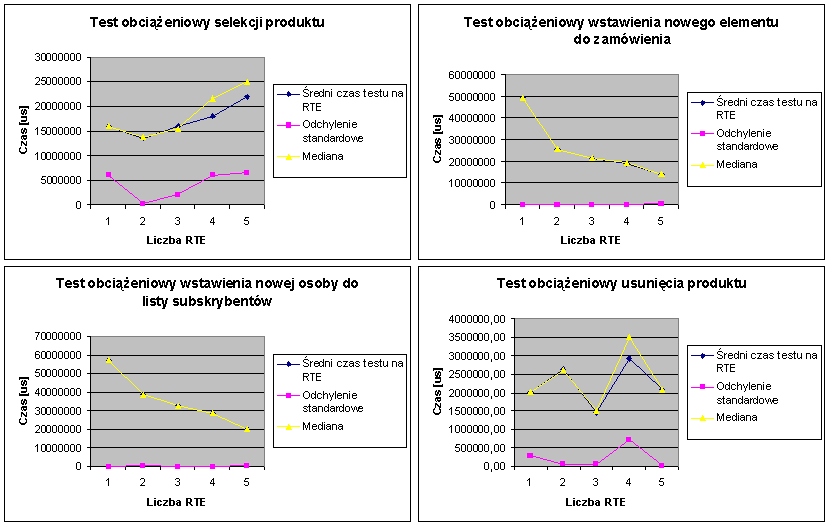
\includegraphics[width=1.1\linewidth]{figures/chart_load.png}
\end{center}
\caption{Wykresy dla testów obciążeniowych}\label{rys:chart_load}
\end{figure}

\begin{figure}[p]
\begin{center}
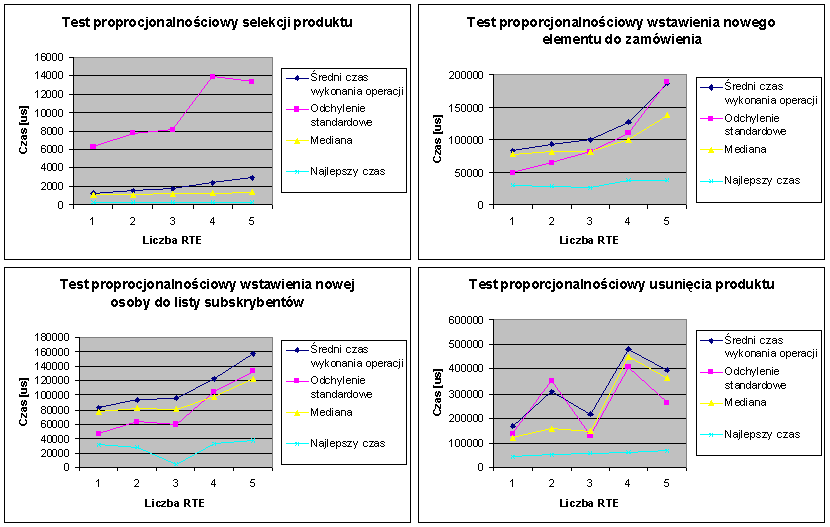
\includegraphics[width=1.1\linewidth]{figures/chart_prop.png}
\end{center}
\caption{Wykresy dla testów proporcjonalnościowych}\label{rys:chart_prop}
\end{figure}


